\clearpage
\subsection{Worked central differences for parts (d)--(f)}
At the common starting point $(0.1,0.01)$ m, the prescribed perturbations are
$\delta_1=0.001$ m and $\delta_2=0.0001$ m. Direct substitution in the
original potential energy gives the values below. Retaining extra digits
is necessary when subtracting nearly equal energy values.
\begin{table}[H]
\centering
\caption{Objective evaluations for the initial central-difference stencil.}
\begin{tabular}{rrr}
\toprule
$x_1$ (m)&$x_2$ (m)&$f$ (J)\\
\midrule
0.100&0.0100&$-694.144789297752$\\
0.101&0.0100&$-699.332880432427$\\
0.099&0.0100&$-688.922149278469$\\
0.100&0.0101&$-693.657151849739$\\
0.100&0.0099&$-694.622599507476$\\
0.101&0.0101&$-698.845242984414$\\
0.101&0.0099&$-699.810690642151$\\
0.099&0.0101&$-688.434511830456$\\
0.099&0.0099&$-689.399959488193$\\
\bottomrule
\end{tabular}
\end{table}
The gradient components follow from the two opposite evaluations in
each coordinate:
\begin{align*}
g_1&\approx\frac{-699.332880432427-(-688.922149278469)}{0.002}
=-5205.365577\ \mathrm N,\\
g_2&\approx\frac{-693.657151849739-(-694.622599507476)}{0.0002}
=4827.238289\ \mathrm N.
\end{align*}
The diagonal second derivatives are
\begin{align*}
H_{11}&\approx
\frac{-699.332880432427-2(-694.144789297752)-688.922149278469}{(0.001)^2}\\
&=34548.8846\ \mathrm{N/m},\\
H_{22}&\approx
\frac{-693.657151849739-2(-694.144789297752)-694.622599507476}{(0.0001)^2}\\
&=982723.8289\ \mathrm{N/m}.
\end{align*}
The mixed stencil is
\[
H_{12}\approx
\frac{f_{++}-f_{+-}-f_{-+}+f_{--}}{4\delta_1\delta_2}\approx0,
\]
where the signs indicate the two coordinate perturbations. The mixed
derivative is exactly zero for this separable quadratic. Thus
$\|\bm g^{(0)}\|_2=7099.159$ N and the diagonal Hessian supplies the
curvatures for Newton and Marquardt. At every subsequent iterate, recompute
the perturbations and the central differences using the current coordinates.

\clearpage
\subsection{Worked steepest-descent and Newton updates}
\paragraph{Steepest descent, part (d).}
The direction and trial point are
\[
\bm p=-\bm g=
\begin{bmatrix}5205.365577\\-4827.238289\end{bmatrix},
\qquad
\bm x(\alpha)=
\begin{bmatrix}0.1+5205.365577\alpha\\0.01-4827.238289\alpha\end{bmatrix}.
\]
The direct line search starts on $[0,1]$. At each round it evaluates the
left quarter point, midpoint and right quarter point with the original
objective, retains the half containing the lowest value, and returns the
final interval midpoint once its width is below $10^{-4}$. The exact line
minimum is $\alpha_*=2.1143863\times10^{-6}$, far smaller than the first
returned midpoint. After 14 rounds the interval is
$[0,6.10352\times10^{-5}]$ and the returned midpoint is
$\alpha=3.05176\times10^{-5}$. Direct evaluation gives
$f(\bm x^{(1)})\approx8867.23$ J, up from $-694.14$ J. The method therefore
accepts an uphill step. Repeating the stated procedure leads to overflow;
the first nonfinite state occurs at iteration 103, so this run diverges
before the limit $M=200$.

As a separate direction-scaling case, use
$\bm p=-\bm g/\|\bm g\|_2$ with the same $[0,1]$ interval, width and cap.
Here $\alpha$ has units of metres. This removes the huge scale of the raw
gradient direction and produces a useful path, but at iteration 200 the
run is still above tolerance, with $\|\bm g\|_2\approx18.57$ N. It is
reported as capped, not converged. The finer, extended runs are parameter
sensitivity cases and are not substituted for the prescribed baseline.

\paragraph{Newton, part (e).}
Solving $H\bm p=-\bm g$ gives
\[
p_1=\frac{5205.365577}{34548.8846}=0.1506666752\ \mathrm m,
\qquad
p_2=\frac{-4827.238289}{982723.8289}=-0.0049121006\ \mathrm m.
\]
The direct interval search returns $\alpha=1-2^{-15}$. After the first
update, the next Newton direction has norm $4.60\times10^{-6}$ m, below
the lecture step tolerance. The point is $(0.2506620773,0.0050880493)$ m
and the residual gradient is $0.21665$ N.

\clearpage
\subsection{Worked Marquardt update and displacement paths}
\paragraph{Marquardt, part (f).}
At $\lambda_0=1000$ N/m, the first trial is
$\bm x=(0.24642838,\,0.00509289)^T$ m. Its directly evaluated energy
is $-1097.827976$ J, below the starting value. Accept it and set
$\lambda=500$ N/m. On each rejection retain the current point and double
$\lambda$; on each acceptance halve it. With this lecture-note rule and
direct objective comparisons, the run reaches the gradient tolerance after
eight trials, with five accepted updates. Three trials near the solution
are rejected when the directly evaluated energy fails the strict decrease test.
\begin{table}[H]
\centering
\caption{Selected direct-evaluation Marquardt iterates.}
\begin{tabular}{rrrr}
\toprule
$k$&$x_1$ (m)&$x_2$ (m)&$\|\bm g\|_2$ (N)\\
\midrule
0&0.1000000000&0.0100000000&$7099.159$\\
1&0.2464283798&0.0050928928&$146.511$\\
2&0.2506062126&0.0050879020&$2.089$\\
3&0.2506662409&0.0050878994&$1.501\times10^{-2}$\\
4&0.2506666737&0.0050878994&$5.410\times10^{-5}$\\
8&0.2506666752&0.0050878994&$7.718\times10^{-7}$\\
\bottomrule
\end{tabular}
\end{table}
\begin{figure}[H]
\centering
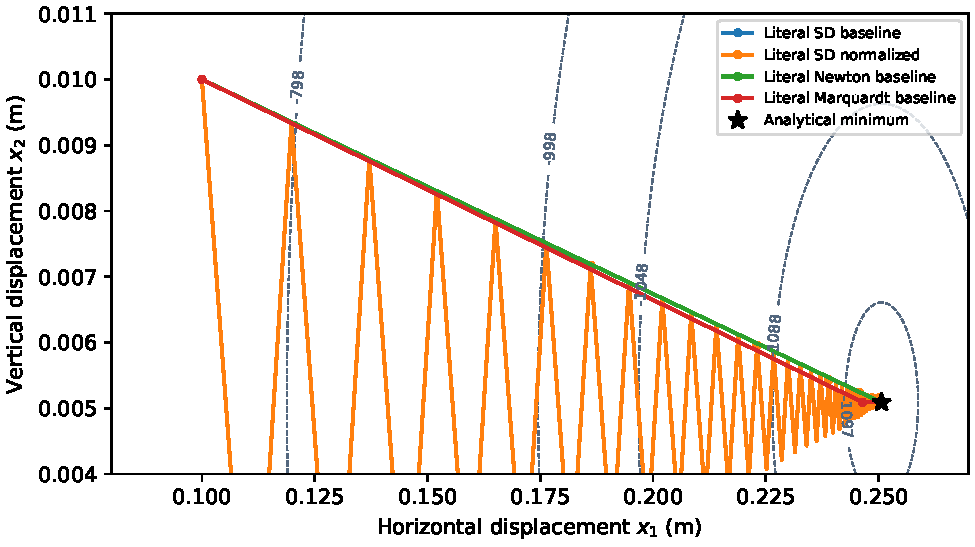
\includegraphics[width=.85\textwidth]{baseline_detail.pdf}
\caption{Magnified baseline displacement paths for parts (d)--(f). Newton meets the lecture step test after one update, while Marquardt meets
the gradient test after eight trials. The normalized
steepest-descent path is shown here; the unnormalized direct run diverges.
The full-window paths appear in the baseline comparison.}
\end{figure}
For part (c), the analytical point is marked on the full contour plot and
the positive-definite Hessian proves the minimum. The displacement paths
provide the iteration diagrams requested for parts (d)--(f).
